% !TEX program = xelatex
% !TeX program = xelatex
\documentclass[12pt,a4paper]{article}
\usepackage[UTF8, heading=true]{ctex}
\usepackage{geometry}
\usepackage{multirow}
\usepackage{booktabs}
\usepackage{graphicx}
\usepackage{float}
\usepackage{listings}
\usepackage{tikz}
\usetikzlibrary{shapes.geometric, arrows, positioning, calc}
\lstset{
    basicstyle=\small\ttfamily,
    breaklines=true,
    columns=flexible,
    keepspaces=true
}
% 页边距设置
\geometry{left=2.5cm,right=2.5cm,top=2.5cm,bottom=2.5cm}
% 字体与行距设置
\ctexset{
    section = { format=\bfseries\large },
    subsection = { format=\bfseries\normalsize }
}
\linespread{1.5}
\fontsize{10.5pt}{12pt}\selectfont

\begin{document}
% 标题
\begin{center}
    \textbf{\small 微机实验三子任务-Proteus}
\end{center}

% 基本信息
\noindent
\textbf{成  绩}\hspace{4cm} \textbf{指导教师}：罗志祥 \\
\textbf{专业班级}：光电信息科学与工程202409 \hspace{1cm} \textbf{姓  名}：陈恪瑾 \hspace{1cm} \textbf{学  号}：U202413925 \\
\textbf{联系电话}：18571851291

\section{任务要求}
\subsection{实验目的}
\begin{itemize}
    \item 加深对 51 系列单片机 I/O 口、键盘与数码显示电路工作机制的理解；
    \item 掌握使用 Proteus 仿真工具进行硬件电路加载、联调与结果分析的方法。
\end{itemize}

\subsection{实验内容}
安装 Proteus 仿真软件后，加载配置工程 \texttt{8051\_SOEI.pdsprj}，在给定硬件环境下编写并调试程序。系统需满足以下功能：
\begin{figure}[H]
    \centering
    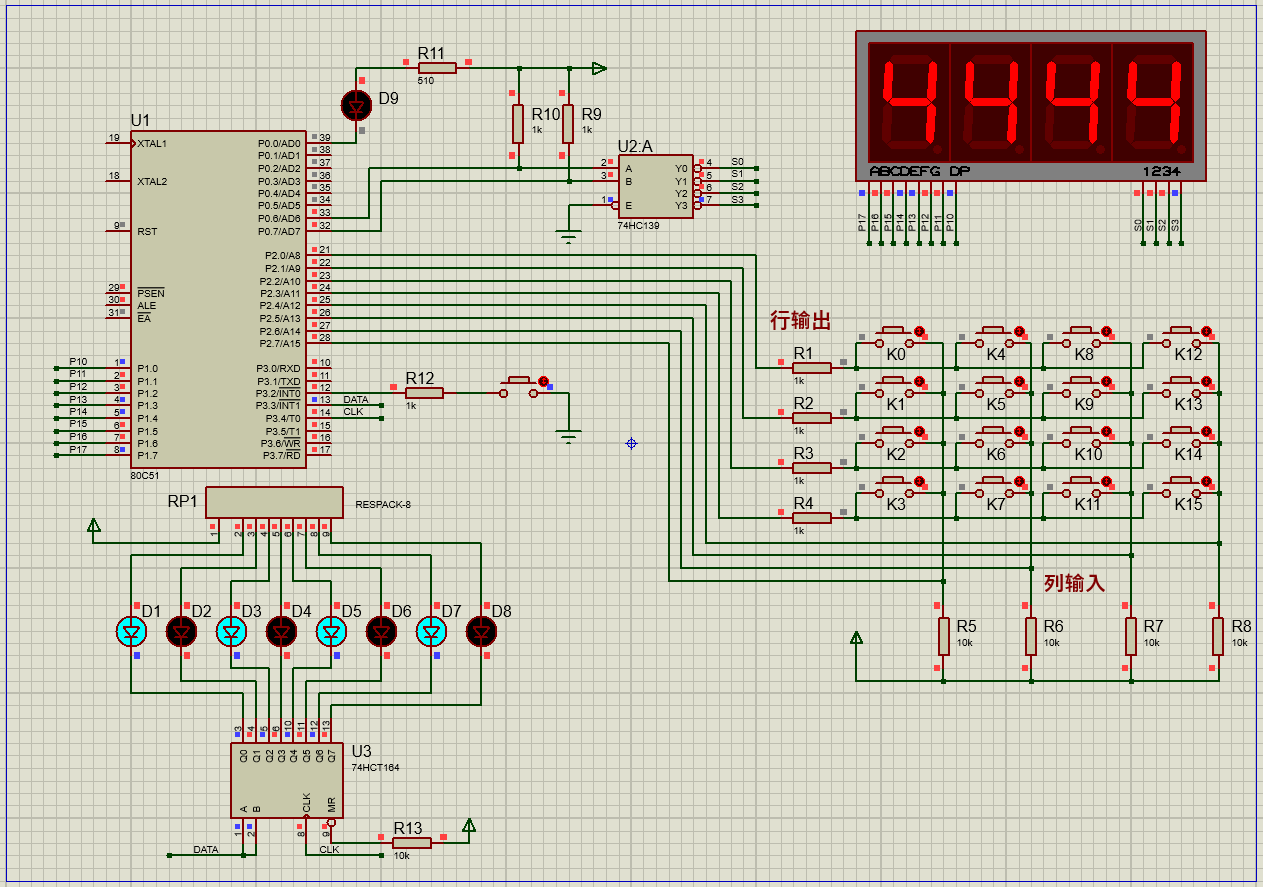
\includegraphics[width=0.82\textwidth]{figures/proteus_env.png}
    \caption{Proteus 仿真硬件环境}
\end{figure}
\begin{itemize}
    \item 在键盘上按下 1、2、3、4 时，任选一个数码管依次显示光电学院英文简称首字母 S、O、E、I；
    \item 显示结果应与键值对应，按键动作与数码管字符变化正确、稳定；
    \item 程序在 Proteus 环境中可正常运行，满足课程实验的基础功能要求。
\end{itemize}
请编写程序，实现键盘输入与数码显示之间的正确逻辑映射。

\subsection{提高部分（申优选做）}
\begin{itemize}
    \item 在键盘上按下 1--4 时，四个数码管逐个点亮并分别显示 S、O、E、I；
    \item 完善多位动态扫描与消隐处理，提升显示稳定性与可读性；
    \item 其他个性化设计。
\end{itemize}

\section{设计思路}
本系统基于 AT89S52 单片机与 Proteus 仿真平台，采用“主循环轮询 + 按键分支处理 + 动态扫描显示”的实现思路。程序以显示缓存（40H$\sim$43H）为核心：按键扫描仅负责更新缓存，数码管刷新子程序持续读取缓存并循环显示，整体设计逻辑如下：
\begin{enumerate}
    \item \textbf{系统初始化模块}：主程序设置堆栈指针 \texttt{SP=5FH}，并将 40H$\sim$43H 显示缓存清零（\texttt{SEG\_OFF}），初始状态为四位全灭；44H 作为按键状态标志清零。
    \item \textbf{主循环调度模块}：\texttt{MAIN\_LOOP} 中循环调用 \texttt{KEY\_SCAN} 与 \texttt{DISPLAY}。其中 \texttt{KEY\_SCAN} 负责识别按键并更新显示数据，\texttt{DISPLAY} 负责一次完整的四位动态刷新。
    \item \textbf{键盘扫描与分支判定模块}：程序通过 \texttt{P2=0FEH} 扫描第 1 行，读取列线 \texttt{ACC.4$\sim$ACC.7} 判定按键。检测到按键后进入 \texttt{KEY\_1\_PRESSED} 至 \texttt{KEY\_4\_PRESSED} 分支；无按键时保持当前缓存不变直接返回。
    \item \textbf{显示内容组织模块}：四个按键采用前缀累积显示策略而非单字符映射。按下 1 显示 ``S''；按下 2 显示 ``SO''；按下 3 显示 ``SOE''；按下 4 显示 ``SOEI''。每次按键先清空 40H$\sim$43H，再写入对应段码常量 \texttt{SEG\_S/SEG\_O/SEG\_E/SEG\_I}。
    \item \textbf{K12 渐进显示模块}：在 \texttt{KEY\_4\_PRESSED} 中，若 44H 标志满足条件则调用 \texttt{STEP\_DELAY} 实现 S$\rightarrow$SO$\rightarrow$SOE$\rightarrow$SOEI 的逐步点亮过程，并在结束后执行一次清屏；否则直接稳定显示 ``SOEI''。
    \item \textbf{动态扫描显示模块}：\texttt{DISPLAY} 子程序使用 \texttt{P0.6/P0.7} 控制 74HC139 位选，按 ``00/01/10/11'' 依次刷新四位；段码由 \texttt{P1} 输出。位切换前先写 \texttt{SEG\_OFF} 消隐，并配合 \texttt{DELAY\_1MS} 降低重影，保证显示稳定。
\end{enumerate}

\section{资源分配}
\subsection{I/O口硬件资源分配}
\begin{table}[H]
    \centering
    \small
    \begin{tabular}{|c|c|c|c|}
        \hline
        I/O引脚 & 方向 & 功能定义 & 有效电平 \\
        \hline
        P1.0$\sim$P1.7 & 输出 & 数码管段码输出（A$\sim$DP） & 高电平点亮，低电平熄灭 \\
        \hline
        P0.6 & 输出 & 位选地址线 0 & 低/高电平配合译码选通 \\
        \hline
        P0.7 & 输出 & 位选地址线 1 & 低/高电平配合译码选通 \\
        \hline
        P2.0$\sim$P2.3 & 输出 & 键盘行线扫描 & 低电平有效 \\
        \hline
        P2.4$\sim$P2.7 & 输入 & 键盘列线检测 & 低电平有效 \\
        \hline
        P3 & 未用 & 保留未连接 & - \\
        \hline
    \end{tabular}
\end{table}

\subsection{寄存器资源分配}
\begin{table}[H]
    \centering
    \small
    \begin{tabular}{|c|c|}
        \hline
        寄存器 & 功能定义 \\
        \hline
        SP & 堆栈指针，初始化为 \texttt{5FH} \\
        \hline
        A & 键盘扫描、位操作与段码装载的累加器 \\
        \hline
        R5 & \texttt{STEP\_DELAY} 过程中的循环计数器 \\
        \hline
        R6 & \texttt{DELAY\_1MS} 的内层延时计数器 \\
        \hline
        R7 & \texttt{DELAY\_1MS} 的外层延时计数器 \\
        \hline
    \end{tabular}
\end{table}

\subsection{片内RAM资源分配}
\begin{table}[H]
    \centering
    \small
    \begin{tabular}{|c|c|}
        \hline
        存储单元 & 功能定义 \\
        \hline
        40H & 第1位数码管显示缓存，保存段码 \texttt{SEG\_S} 等 \\
        \hline
        41H & 第2位数码管显示缓存，保存段码 \texttt{SEG\_O} 等 \\
        \hline
        42H & 第3位数码管显示缓存，保存段码 \texttt{SEG\_E} 等 \\
        \hline
        43H & 第4位数码管显示缓存，保存段码 \texttt{SEG\_I} 等 \\
        \hline
        44H & 显示状态标志，用于控制 \texttt{KEY\_4\_PRESSED} 的渐进显示分支 \\
        \hline
    \end{tabular}
\end{table}

\section{流程图}
\subsection{主程序流程图}
\begin{figure}[H]
    \centering
    \small
    \begin{tikzpicture}[node distance=1.0cm, scale=0.85, transform shape]
        \tikzstyle{startstop} = [rectangle, rounded corners, minimum width=2.8cm, minimum height=0.8cm, text centered, align=center, draw=black, fill=red!10]
        \tikzstyle{process} = [rectangle, minimum width=4.3cm, minimum height=0.8cm, text centered, align=center, draw=black, fill=blue!10]
        \tikzstyle{arrow} = [thick,->,>=stealth]

        \node (start) [startstop] {开始};
        \node (init) [process, below=of start] {SP=5FH\\40H$\sim$43H清零，44H=00H};
        \node (loop) [process, below=of init] {MAIN\_LOOP};
        \node (key) [process, below=of loop] {调用 KEY\_SCAN};
        \node (disp) [process, below=of key] {调用 DISPLAY};
        \node (back) [process, below=of disp] {返回主循环};

        \draw [arrow] (start) -- (init);
        \draw [arrow] (init) -- (loop);
        \draw [arrow] (loop) -- (key);
        \draw [arrow] (key) -- (disp);
        \draw [arrow] (disp) -- (back);
        \draw [arrow] (back.east) -- ++(2.0,0) |- (loop.east);
    \end{tikzpicture}
    \caption{主程序流程图}
\end{figure}

\subsection{按键扫描流程图}
\begin{figure}[H]
    \centering
    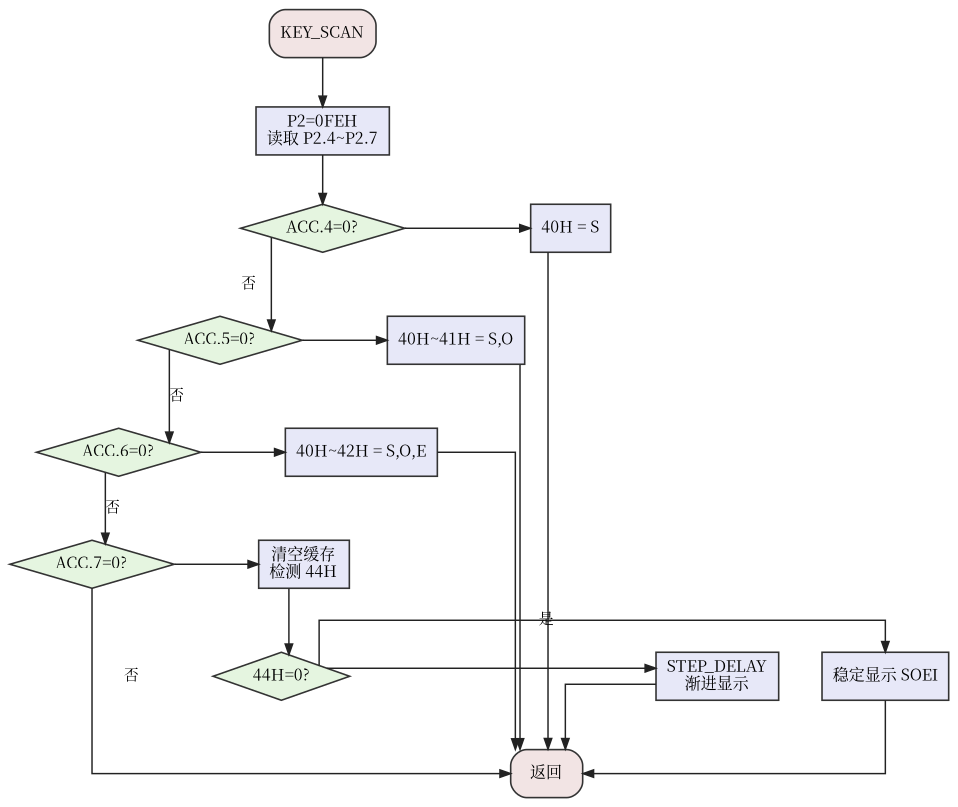
\includegraphics[width=0.96\textwidth]{figures/key_scan_flow.png}
    \caption{按键扫描流程图}
\end{figure}

\subsection{数码管动态刷新流程图}
\begin{figure}[H]
    \centering
    \small
    \begin{tikzpicture}[node distance=1.0cm, scale=0.85, transform shape]
        \tikzstyle{startstop} = [rectangle, rounded corners, minimum width=2.8cm, minimum height=0.8cm, text centered, align=center, draw=black, fill=red!10]
        \tikzstyle{process} = [rectangle, minimum width=4.5cm, minimum height=0.8cm, text centered, align=center, draw=black, fill=blue!10]
        \tikzstyle{arrow} = [thick,->,>=stealth]

        \node (start) [startstop] {DISPLAY};
        \node (d1) [process, below=of start] {P1=SEG\_OFF\\P0.6/P0.7=00\\P1=40H};
        \node (d2) [process, below=of d1] {P1=SEG\_OFF\\P0.6/P0.7=01\\P1=41H};
        \node (d3) [process, below=of d2] {P1=SEG\_OFF\\P0.6/P0.7=10\\P1=42H};
        \node (d4) [process, below=of d3] {P1=SEG\_OFF\\P0.6/P0.7=11\\P1=43H};
        \node (ret) [startstop, below=of d4] {返回};

        \draw [arrow] (start) -- (d1);
        \draw [arrow] (d1) -- (d2);
        \draw [arrow] (d2) -- (d3);
        \draw [arrow] (d3) -- (d4);
        \draw [arrow] (d4) -- (ret);
    \end{tikzpicture}
    \caption{数码管动态刷新流程图}
\end{figure}

\subsection{渐进显示流程图}
\begin{figure}[H]
    \centering
    \small
    \begin{tikzpicture}[node distance=1.05cm, scale=0.85, transform shape]
        \tikzstyle{startstop} = [rectangle, rounded corners, minimum width=2.8cm, minimum height=0.8cm, text centered, align=center, draw=black, fill=red!10]
        \tikzstyle{process} = [rectangle, minimum width=4.4cm, minimum height=0.8cm, text centered, align=center, draw=black, fill=blue!10]
        \tikzstyle{decision} = [diamond, aspect=2.0, minimum width=3.2cm, minimum height=0.9cm, text centered, align=center, draw=black, fill=green!10]
        \tikzstyle{arrow} = [thick,->,>=stealth]

        \node (start) [startstop] {STEP\_DELAY};
        \node (init) [process, below=of start] {R5=80H};
        \node (disp) [process, below=of init] {调用 DISPLAY};
        \node (dec) [process, below=of disp] {R5--};
        \node (q) [decision, below=of dec] {R5$\neq$0?};
        \node (ret) [startstop, below=of q] {返回};

        \draw [arrow] (start) -- (init);
        \draw [arrow] (init) -- (disp);
        \draw [arrow] (disp) -- (dec);
        \draw [arrow] (dec) -- (q);
        \draw [arrow] (q.west) -- ++(-1.5,0) |- node[pos=0.2,left] {是} (disp.west);
        \draw [arrow] (q) -- node[right] {否} (ret);
    \end{tikzpicture}
    \caption{渐进显示流程图}
\end{figure}

\section{源代码 （含文件头说明、语句行注释）}
\lstinputlisting[language={[x86masm]Assembler}]{codes/STARTUP.asm}

\section{程序测试方法与结果}
本节在 Proteus 仿真环境下对显示功能进行验证，重点检查按键输入与四位数码管显示结果是否一致。

\subsection{测试方法}
\begin{enumerate}
    \item \textbf{初始化测试}：复位后观察四位数码管是否全部熄灭。
    \item \textbf{按键功能测试}：依次触发按键 1、2、3、4，观察显示是否依次为 S、SO、SOE、SOEI。
    \item \textbf{稳定性测试}：保持按键释放状态，观察显示是否稳定无异常跳变。
\end{enumerate}

\subsection{测试结果}
\textbf{（1）数码管空显示测试}

操作：系统上电复位，不按任何按键。\\
预期：四位数码管均不显示字符。\\
结果：与预期一致。

\begin{figure}[H]
    \centering
    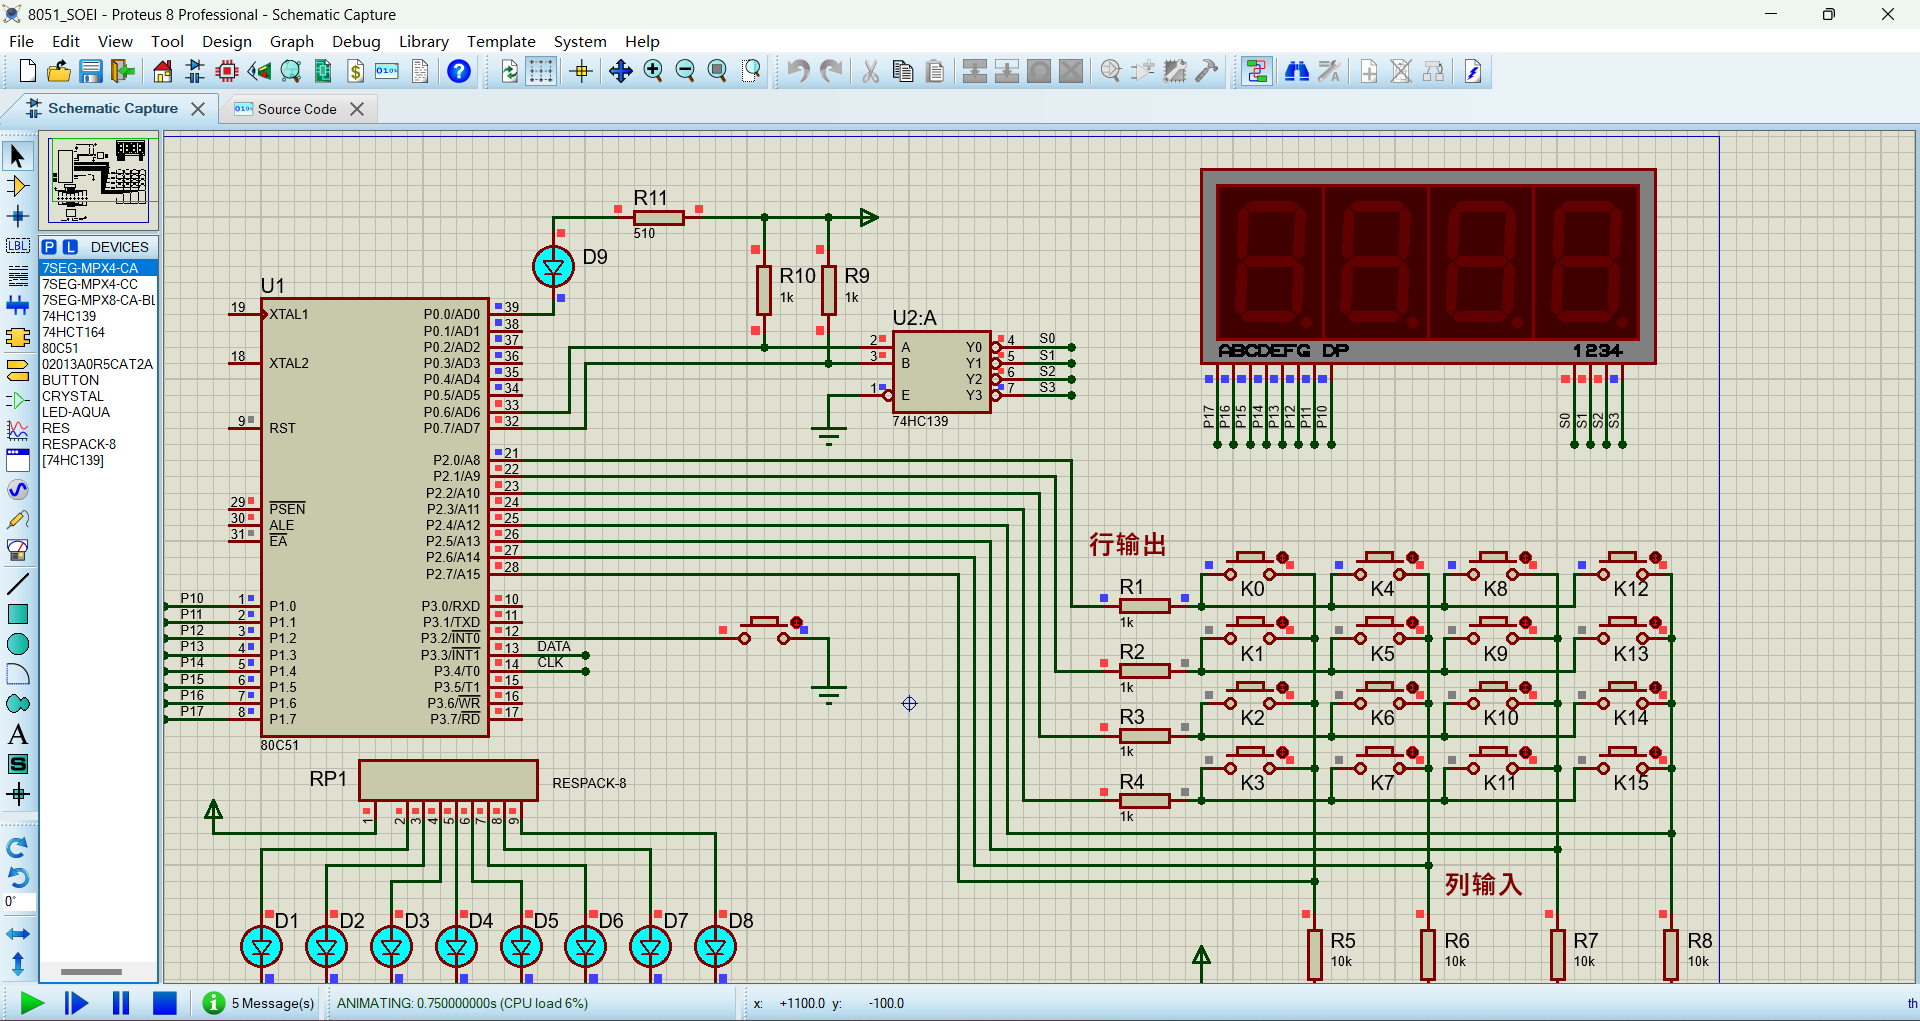
\includegraphics[width=0.78\textwidth]{figures/figure1.png}
    \caption{空显示测试结果}
\end{figure}

\textbf{（2）显示 S 测试}

操作：按下按键 1。\\
预期：数码管显示 S。\\
结果：与预期一致。

\begin{figure}[H]
    \centering
    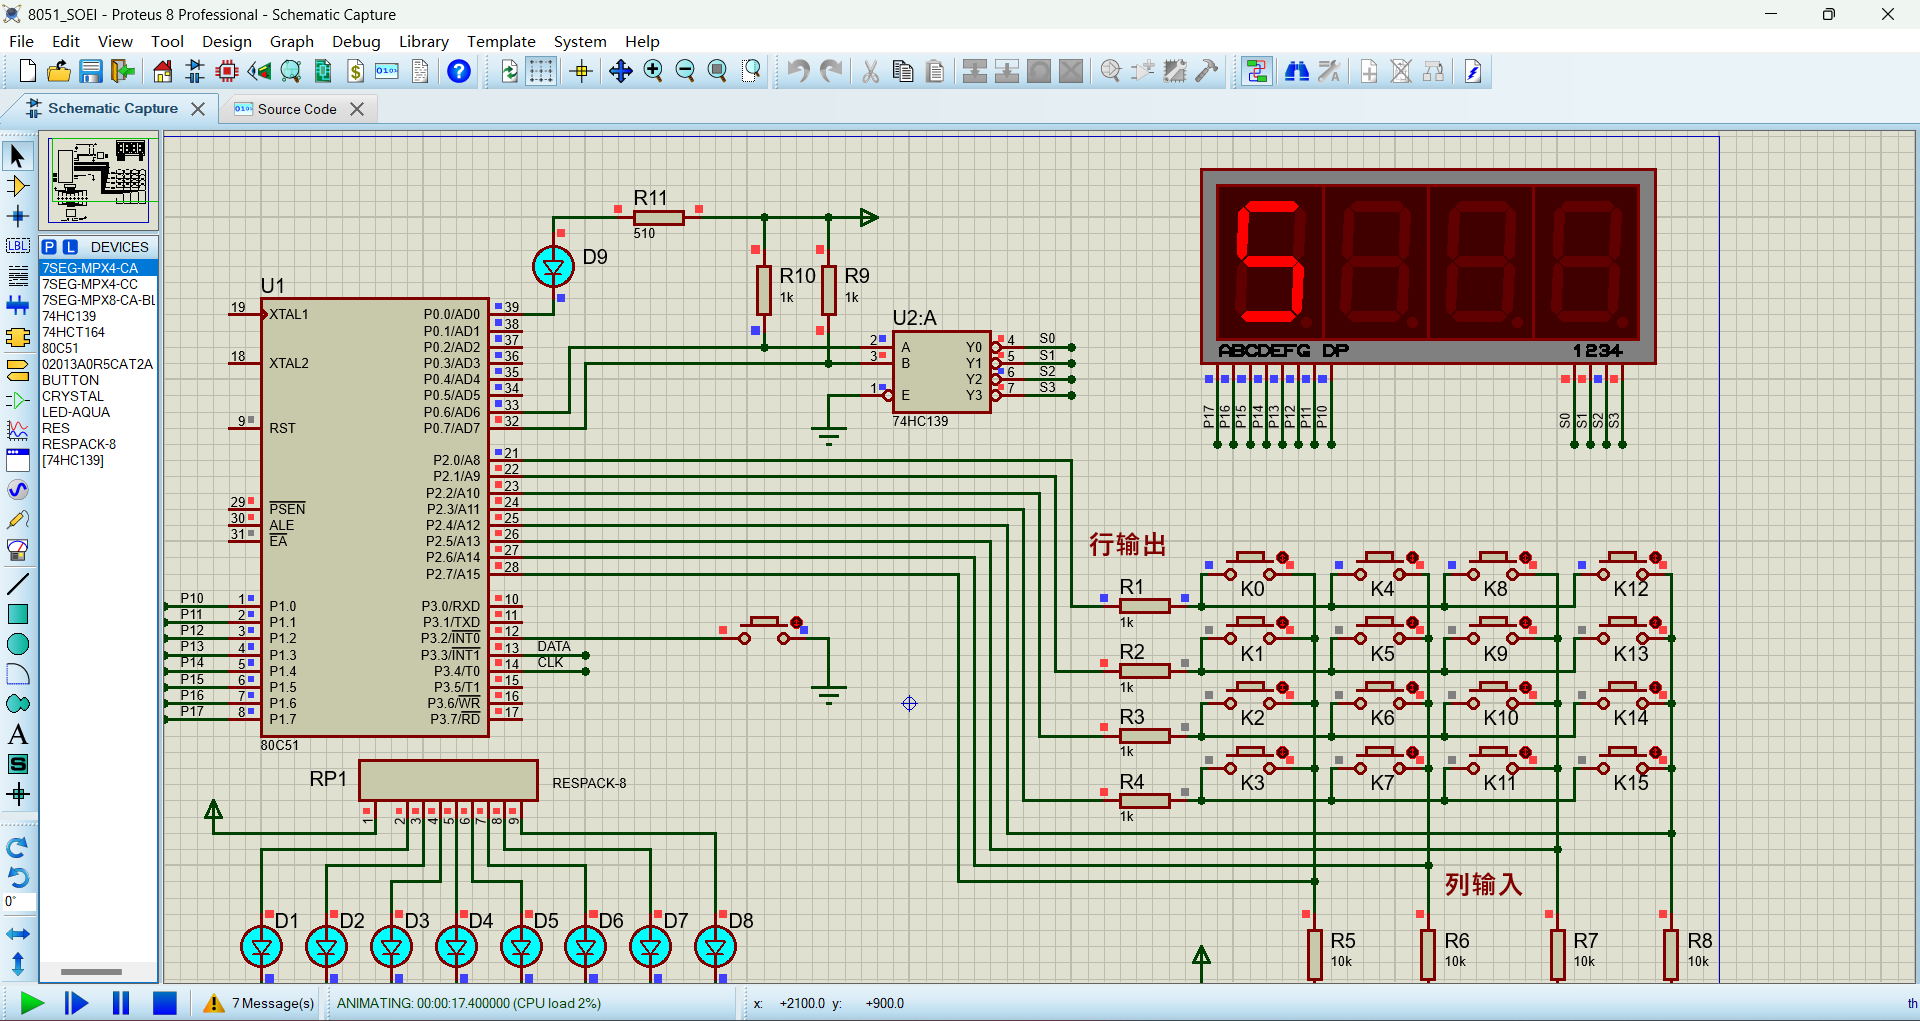
\includegraphics[width=0.78\textwidth]{figures/figure2.png}
    \caption{显示 S 测试结果}
\end{figure}

\textbf{（3）显示 SO 测试}

操作：按下按键 2。\\
预期：数码管显示 SO。\\
结果：与预期一致。

\begin{figure}[H]
    \centering
    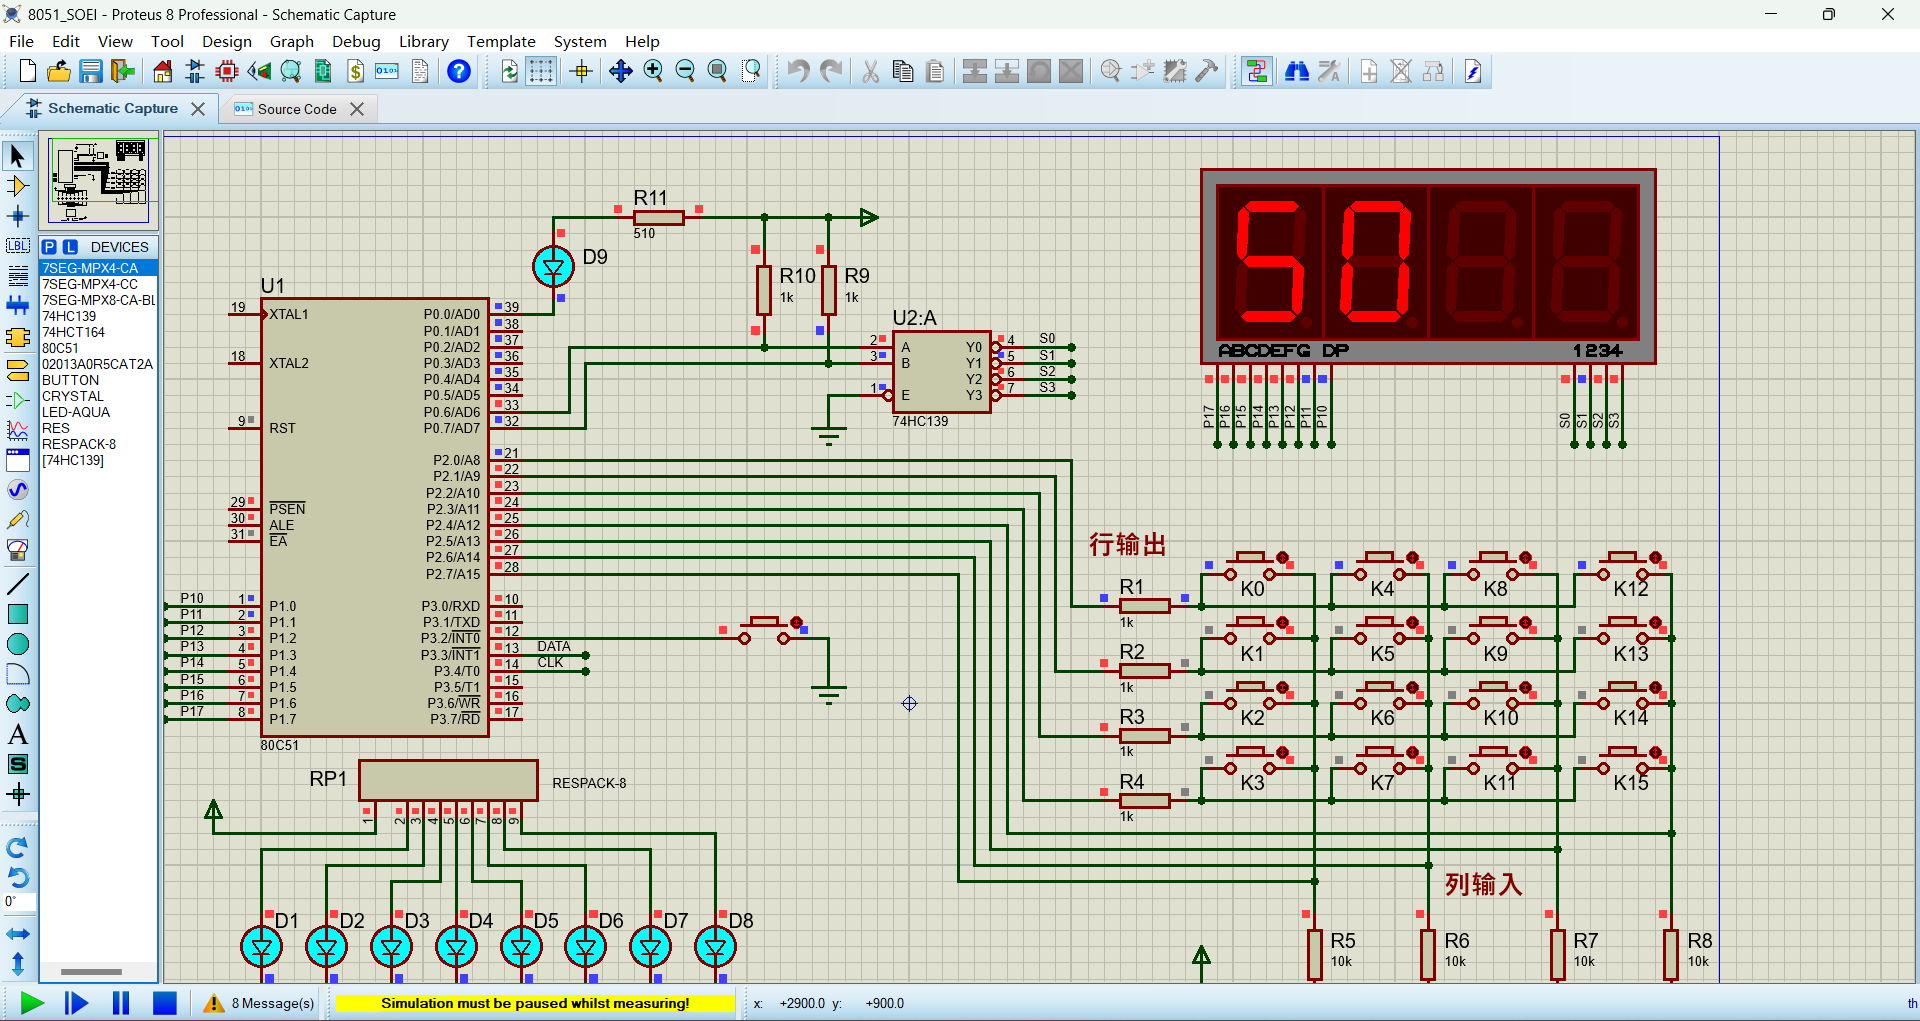
\includegraphics[width=0.78\textwidth]{figures/figure3.png}
    \caption{显示 SO 测试结果}
\end{figure}

\textbf{（4）显示 SOE 测试}

操作：按下按键 3。\\
预期：数码管显示 SOE。\\
结果：与预期一致。

\begin{figure}[H]
    \centering
    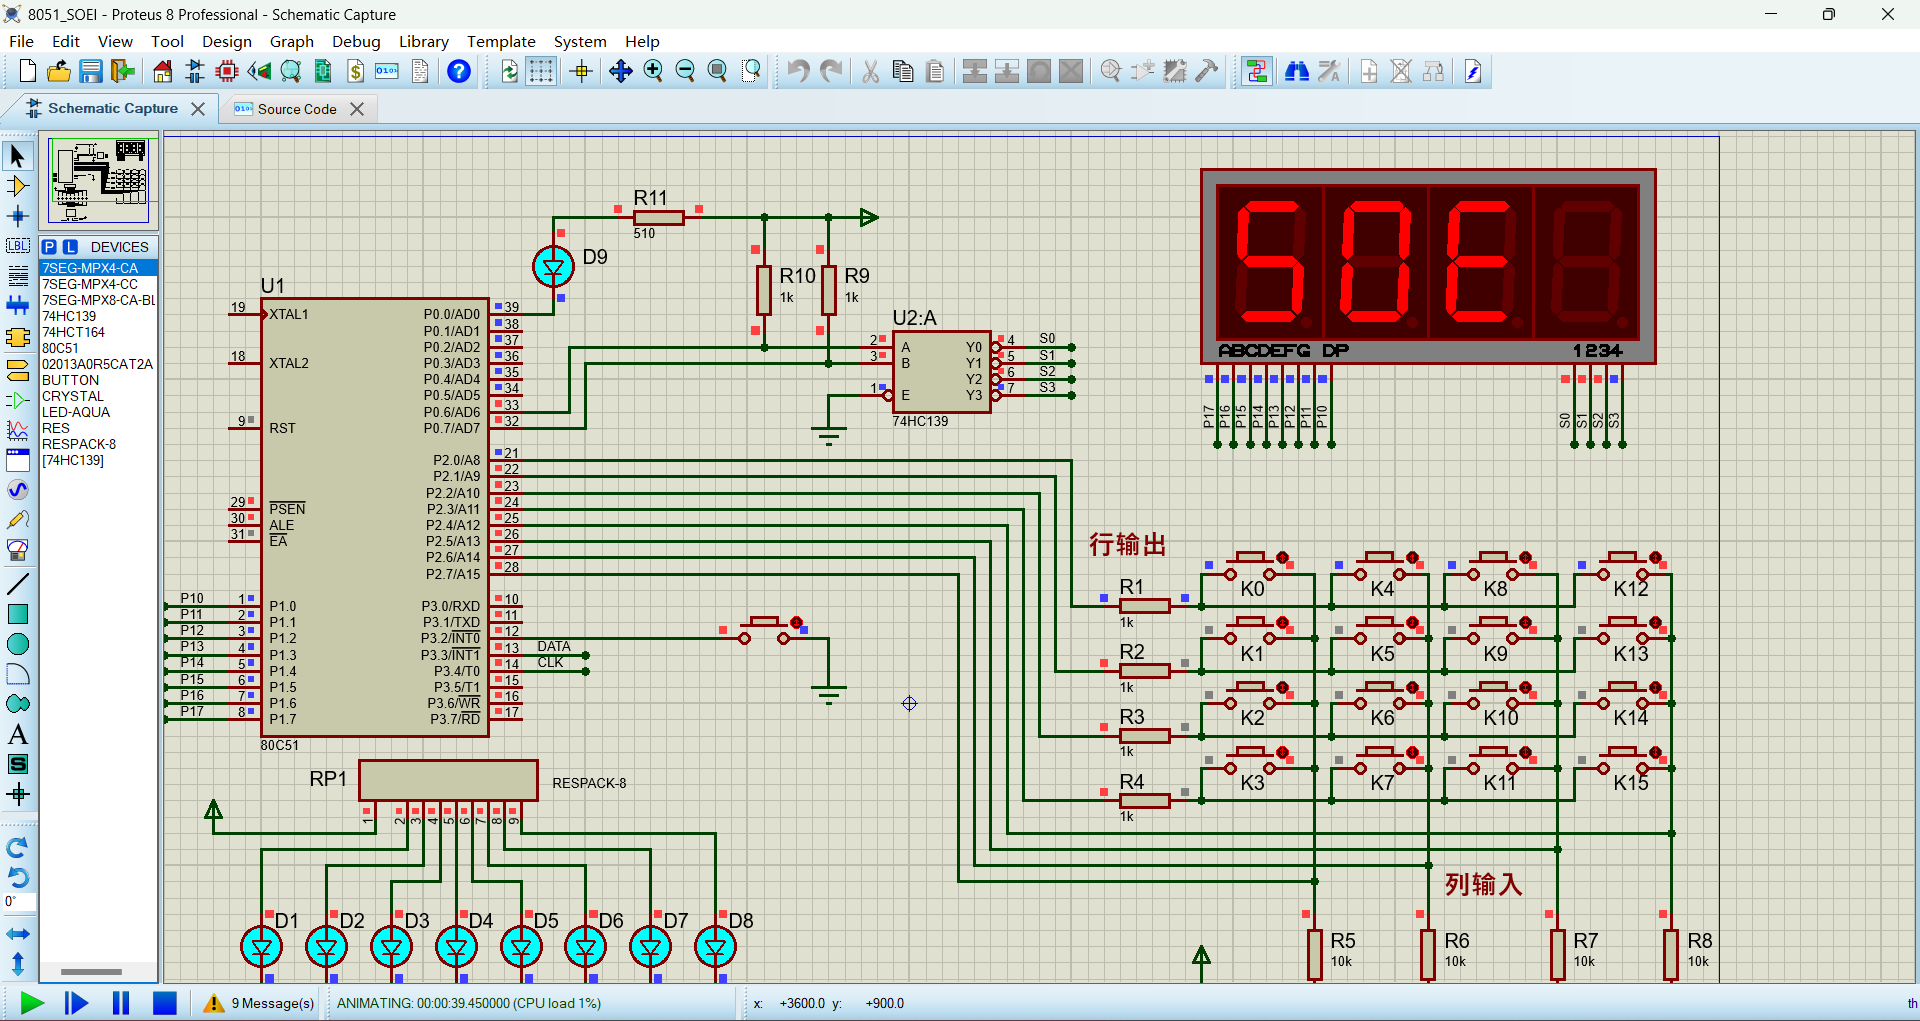
\includegraphics[width=0.78\textwidth]{figures/figure4.png}
    \caption{显示 SOE 测试结果}
\end{figure}

\textbf{（5）显示 SOEI 测试}

操作：按下按键 4。\\
预期：数码管显示 SOEI。\\
结果：与预期一致。

\begin{figure}[H]
    \centering
    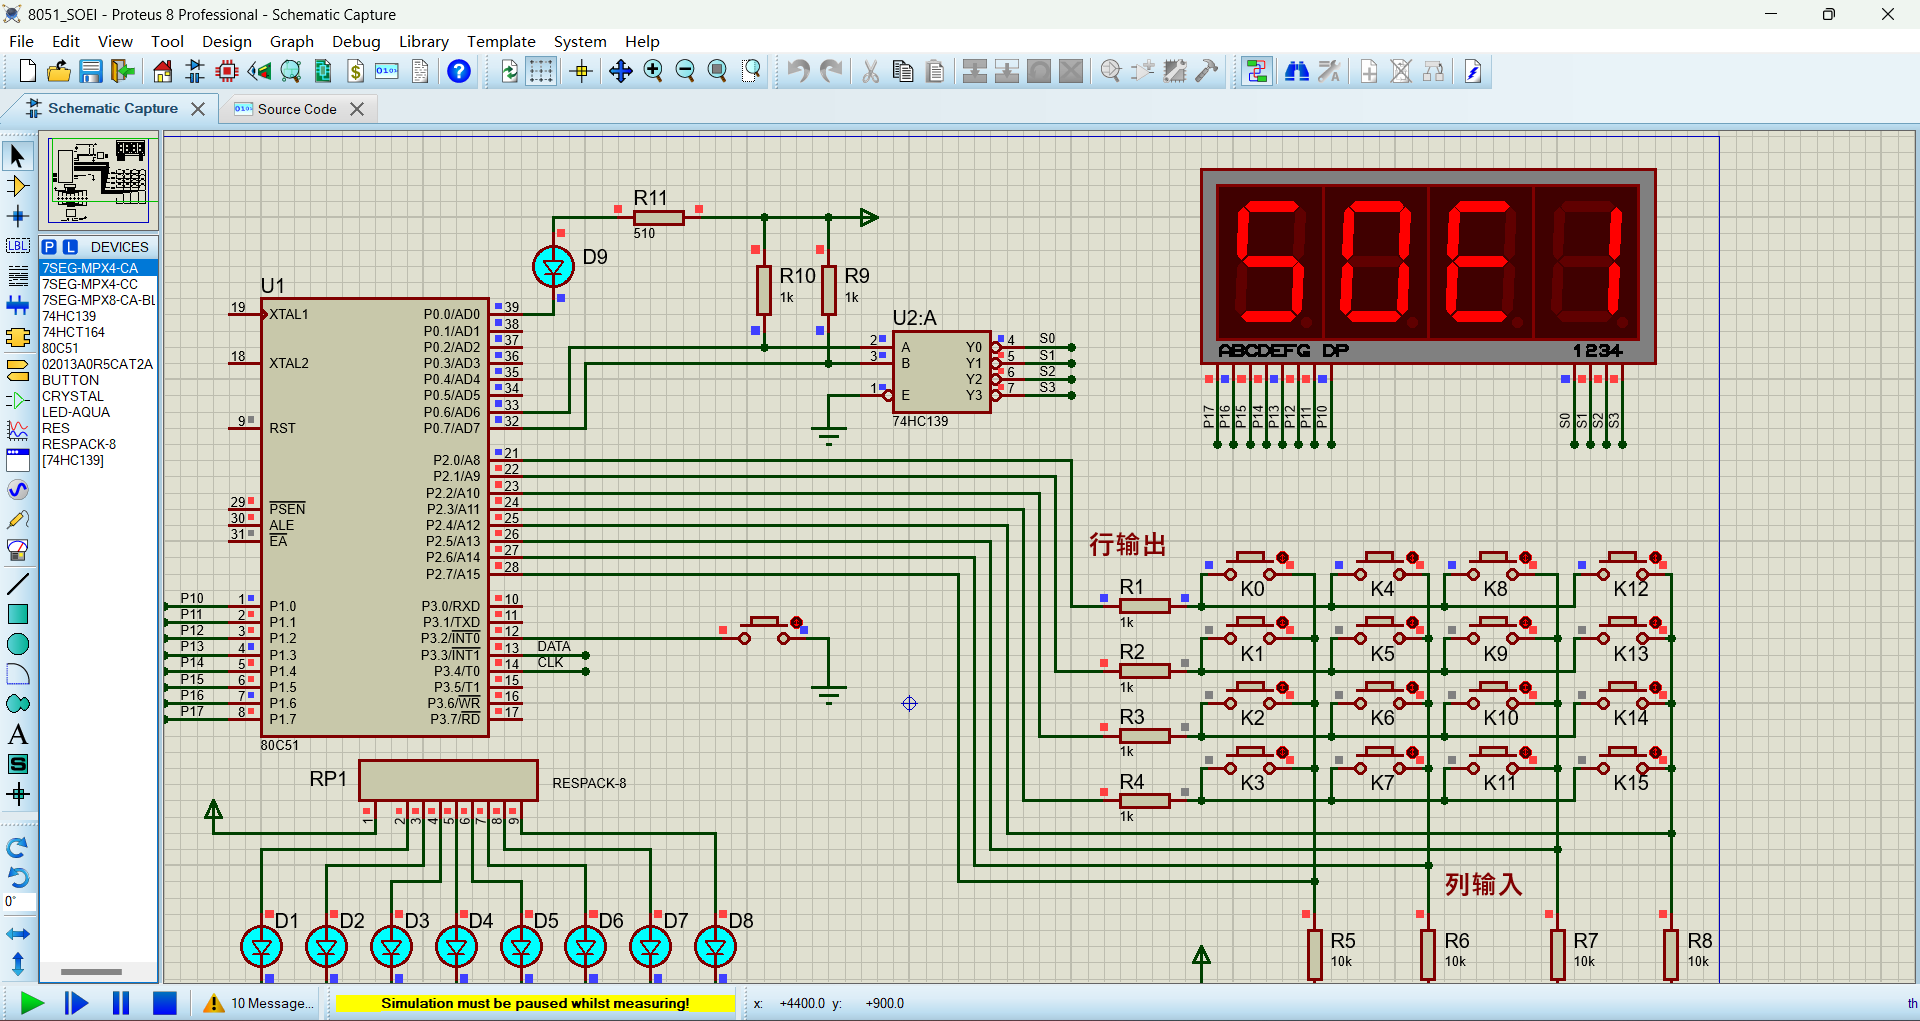
\includegraphics[width=0.78\textwidth]{figures/figure5.png}
    \caption{显示 SOEI 测试结果}
\end{figure}

综上，程序已完成任务书要求的显示功能：在不同按键输入下，数码管能够稳定输出空显示、S、SO、SOE、SOEI 五种状态。




\section{实验问题分析与对策}

\begin{enumerate}
    \item \textbf{数码管显示字形与预期不符}：
    \begin{itemize}
        \item \textbf{原因分析}：段码与电路接线顺序不匹配，导致各段点亮错误。
        \item \textbf{对策}：对照原理图逐一确认 P1.0$\sim$P1.7 分别对应 DP、G、F、E、D、C、B、A 引脚，重新计算共阴极段码：S=0B6H、O=0FCH、E=09EH、I=060H，验证后问题解决。
    \end{itemize}
    
    \item \textbf{动态扫描出现重影}：
    \begin{itemize}
        \item \textbf{原因分析}：切换位选时未先消隐，导致段码残留驱动了下一位数码管。
        \item \textbf{对策}：在 \texttt{DISPLAY} 子程序中，每次切换位选前先向 P1 写入 \texttt{SEG\_OFF}（0x00）进行消隐，再设置位选和段码，消除了重影现象。
    \end{itemize}

    \item \textbf{按键4逐步点亮动画过快，肉眼无法看清}：
    \begin{itemize}
        \item \textbf{原因分析}：单纯使用软件延时循环期间停止了动态显示，导致实际延时不足或显示闪烁。
        \item \textbf{对策}：将 \texttt{STEP\_DELAY} 改为内部循环调用 \texttt{DISPLAY} 子程序约 80 次，在延时过程中持续刷新显示，动画效果流畅且无闪烁。
    \end{itemize}

    \item \textbf{重复按下按键4时动画不触发}：
    \begin{itemize}
        \item \textbf{原因分析}：44H 标志位在动画结束后未正确复位，导致第二次按下直接跳转至 \texttt{K12\_NO\_DELAY} 分支。
        \item \textbf{对策}：检查逻辑后，将 44H 初始设为 00H，按键 1 按下时置为 01H，按键 4 按下时根据 44H 决定是否执行动画，动画完成后手动清零 44H，保证每次从按键 1$\rightarrow$4 的操作序列均可触发动画。
    \end{itemize}

\end{enumerate}

\vspace{2cm}
\noindent
本人承诺:本报告内容真实，无伪造数据，无抄袭他人成果。本人完全了解学校相关规定，如若违反，愿意承担其后果。

\vspace{1cm}
\noindent
签字：\hspace{3cm} 陈恪瑾 \hspace{3cm} 2026年4月26日

\end{document}
